\subsection{Theory of our implementation}

When we want to project a box onto different surfaces, we need to
calculate new camera parameters K * [I | O] each time we change
scene/angle. Some parameters can be reused. The intrinsic camera matrix “K”
doesn’t rely on anything from the scene and remains the same once calibrated. 

The first projection and the first camera.
The first camera initialized in our implementation uses the the fact that our
camera has been calibrated, and the projection plane is fully frontal and dead
center (in theory).
Therefore, no rotation and no translation in happening in the projection and
the [I | O] part of our camera class is equal to the identity matrix
(changes nothing when multiplied onto another matrix). 

The box cordinates are projected in the center of the image and viewed
directly from above.
As the projection is a perspective projection not a parallel projection, the
box appears realisticly to “pop” out from the surface. 

\begin{figure}[H]
\center
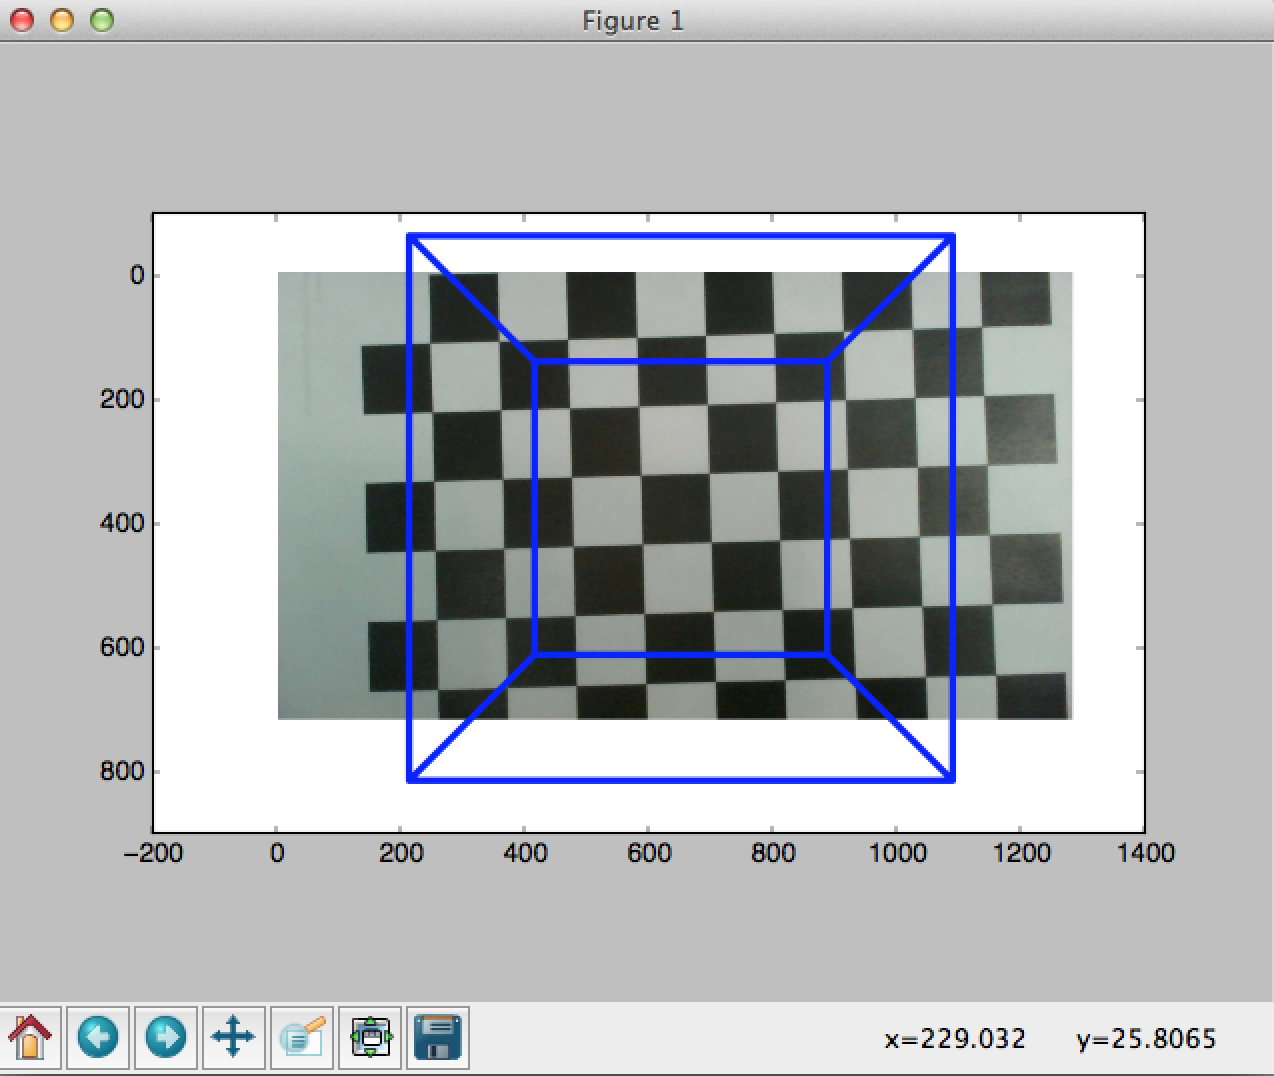
\includegraphics{pics/aug1}
\caption{The first projection onto a fully frontal surface.}
\label{aug1}
\end{figure}

When we want to project the box realistically onto the chessboard when the image
is no longer fully frontal, we calculate a new camera class.
This is done through the following steps:
1.We estimate a homography between the two chessboard surfaces, gaining a 2d
conversion between the two chessboards/scenes.
2.We multiply the existing camera with the homography as using the
homography is a perfectly valid way of projecting the 2D “X” and “Y” coords.
3.We estimate values for the “Z” axis by taking the cross product of the “X”
and “Y” axis-vectors. Thsi will always be orthogonal to both these
vectors, and therefore a good, but not precise estimation of the z-axis.


\begin{figure}[H]
\center
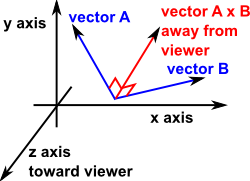
\includegraphics{pics/crossProduct.png}
\caption{Estimating the third axis from the existing two by taking the AxB crossproduct.}
\label{cross_product}
\end{figure}
